\documentclass[wes, manuscript]{copernicus}

\usepackage{amsmath}
\usepackage{graphicx}
\usepackage{booktabs}
\usepackage{float}
%\usepackage{siunitx}  % conflicts with copernicus \unit
% Use \\, manually or plain text for units
\usepackage{natbib}
\usepackage{hyperref}

\title{Design regret in clustered wind farms: how wind rose directionality and optimization thoroughness shape the cost of ignoring neighbors}

\Author[1]{Julian}{Quick}
\Author[2]{Samuel}{Kainz}
\Author[1]{Pierre-Elouan}{R\'ethor\'e}

\affil[1]{Technical University of Denmark, Department of Wind and Energy Systems, Roskilde, Denmark}
\affil[2]{Wind Energy Institute, Technical University of Munich, Germany}

\correspondence{Julian Quick (juqu@dtu.dk)}

\runningtitle{Design regret in clustered wind farms}
\runningauthor{Quick, Kainz, and R\'ethor\'e}

\begin{document}

\maketitle

\begin{abstract}
When a wind farm is designed in isolation---ignoring the wakes of potential neighboring farms---how much energy is sacrificed?
We define this loss as \emph{design regret}: the difference in annual energy production between a layout re-optimized with knowledge of neighbors and the original isolation-designed layout, both evaluated under the same neighbor wakes.
Using two complementary approaches---greedy adversarial placement of individual turbines (upper bound) and regret cross-sections with an identical neighboring farm copy (realistic scenario)---we sweep the two-parameter elliptical wind rose space of Hart (2025).
The adversarial upper bound on regret varies six-fold across wind climate: from 17\,GWh/yr (0.4\,\% of AEP) under bidirectional conditions to 101\,GWh/yr (2.5\,\%) under concentrated unidirectional conditions, with wind rose directionality as the dominant driver.
Regret cross-sections with a realistic identical neighbor farm show substantially lower regret (0.1--0.4\,\% of AEP for multi-directional wind roses), confirming that the adversarial framing overstates risk by roughly an order of magnitude.
A degenerate single-wind-direction stress test produces an order-of-magnitude larger regret (1.25\,\%), presented separately because the multi-directional cases are the realistic scenario.
Critically, reliable regret estimation requires a large multistart budget: we show that regret only stabilizes by $K = 300$ restarts.
We recommend a minimum of 300 multistart optimizations for any study computing AEP differences between design strategies.
\end{abstract}


\section{Introduction}

The North Sea is entering an era of unprecedented wind farm clustering.
Denmark's Vindm\o{}lleparken energy island will connect up to 10\,GW across multiple farms in a shared concession zone; the German Bight already hosts over 8\,GW with plans for 30\,GW by 2050; and the broader North Sea basin is projected to reach 300\,GW as part of Europe's 500\,GW offshore target.
At this density, wind farms no longer operate in isolation.
Cluster wake losses in the German Bight are projected to reduce capacity factors by 30\,\%, with half of the loss attributable to cross-border wake accumulation \citep{Fliegner2025}.
The phenomenon---increasingly termed ``wind theft'' \citep{Finseraas2024, Du2026}---has prompted the UK to issue the first national policy guidance on inter-farm wake effects and NYSERDA to recommend minimum inter-farm spacing of 4\,nmi \citep{NYSERDA2024}.
Wake-induced velocity deficits have been measured at distances exceeding 50\,km \citep{Schneemann2020, Canadillas2022}, and inter-farm losses are projected to exceed the impact of a century of climate change on North Sea wind resources \citep{Warder2025}.

Yet these emerging policy responses share a common gap: they treat all sites uniformly.
Buffer distance recommendations, ``good neighbour'' design principles, and compensation frameworks do not account for variation in wind climate.
This is a significant omission.
A site where wind blows predominantly from one direction creates a single, predictable wake corridor that a neighbor-aware layout can avoid.
A site with bidirectional wind creates competing corridors that no single rearrangement can escape.
The value of coordinated design---and the cost of failing to coordinate---should depend fundamentally on the directional structure of the wind resource.

We formalize this intuition through the concept of \emph{design regret}: the AEP difference between a layout designed with perfect neighbor foresight and one designed in isolation, both evaluated under the same neighbor wakes:
\begin{equation}\label{eq:regret}
    R = \text{AEP}(\mathbf{x}^*_\text{cons}, \mathbf{n}) - \text{AEP}(\mathbf{x}^*_\text{lib}, \mathbf{n}).
\end{equation}
Design regret isolates the cost of the design decision itself, separate from the total AEP reduction caused by neighbor wakes.
By sweeping the elliptical wind rose parameterization of \citet{Hart2025}---which separates directional concentration from bidirectionality---we quantify how wind rose shape governs design regret.
The answer is dramatic: regret varies six-fold across the shape space, from 17\,GWh/yr under bidirectional conditions to 101\,GWh/yr under concentrated unidirectional conditions.
Buffer distance requirements inherit this dependence.

\citet{Quick2026omae} applied this framework to the Danish Energy Island cluster and found negligible design regret for all nine neighbor configurations.
We show this is not a general property of offshore wind, but a consequence of DEI's partially bidirectional wind climate ($f \approx 0.38$).
Sites in the southern North Sea with strongly unidirectional southwesterly winds sit in the high-regret region of the shape space and are substantially more vulnerable to uncoordinated cluster development.

However, accurately computing these quantities reveals a methodological challenge that undermines all existing regret-like calculations.
Layout optimization is highly multimodal \citep{Thomas2023, ValottaRodrigues2024}, and regret---as the \emph{difference} between two optimization outcomes---amplifies the effect of local optima.
We show that at least 300 restarts are needed for the regret estimate to stabilize---over an order of magnitude more than typical practice.

This paper makes four contributions:
\begin{enumerate}
    \item A convergence study demonstrating that 300+ multistart optimizations are needed for reliable regret estimation---over an order of magnitude more than typical practice.
    \item A systematic sweep of the wind rose shape space showing that design regret varies six-fold with directionality, with concentrated unidirectional sites most vulnerable.
    \item Buffer distance analysis quantifying how neighbor separation reduces regret, and how the decay rate depends on wind rose shape.
    \item Regret cross-sections with a realistic identical neighbor farm, showing that design regret is an order of magnitude lower than the adversarial upper bound and peaks in the upwind direction.
\end{enumerate}


\section{Methods}\label{sec:methods}

\subsection{Problem formulation}

We consider a target wind farm of $N_t = 50$ IEA 15\,MW turbines ($D = 240\,m$, hub height 150\,m) within a fixed polygonal boundary derived from the Danish Energy Island concession zone.
Minimum inter-turbine spacing is $4D$ (960\,m).
This configuration is representative of near-future North Sea developments: the IEA 15\,MW turbine is the reference class for planned GW-scale projects, and the DEI polygon provides a realistic, irregular boundary.

The liberal layout $\mathbf{x}^*_\text{lib}$ maximizes AEP assuming no external turbines.
The conservative layout $\mathbf{x}^*_\text{cons}$ maximizes AEP with specified neighbors~$\mathbf{n}$.
Both are evaluated with neighbors present to compute regret via Eq.~\eqref{eq:regret}.
By construction, $R \geq 0$ when both reach global optima.
We enforce this computationally through \emph{regret pooling}: the conservative AEP is taken as $\max(\text{best conservative AEP},\; \text{liberal AEP with neighbors})$, guaranteeing non-negative regret even with imperfect optimization.

\subsection{Wake model}

We use the \citet{Bastankhah2014} Gaussian deficit model with $k = 0.04$ and root-sum-of-squares superposition.
The simulation is implemented in JAX \citep{jax2018github}, enabling automatic differentiation through the wake model.
AEP is computed over 24 equally-spaced wind direction sectors at a constant wind speed of 9\,m/s:
\begin{equation}
    \text{AEP} = 8760 \sum_{k=1}^{24} w_k \sum_{i=1}^{N_t} P_i(U_{i,k}),
\end{equation}
where $w_k$ is the sector frequency, $P_i$ is the turbine power curve, and $U_{i,k}$ is the effective wind speed at turbine $i$ under direction~$k$.

\subsection{Wind rose parameterization}

Wind rose shape is parameterized using the elliptical model of \citet{Hart2025}, which derives the directional frequency distribution from a unit-area ellipse with semi-major axis $a$ (along the prevailing-direction axis) and semi-minor axis $b = 1/(\pi a)$ (perpendicular).
The CDF of a direction $\theta$ relative to the prevailing axis is built from the first-quadrant expression (Hart 2025, Eq.~2):
\begin{equation}\label{eq:hart-cdf-q1}
    F_{Q1}(\theta) = \frac{1}{2\pi}\arctan\!\left(\pi\,a^{2}\,\tan\theta\right), \qquad \theta \in [0, \pi/2),
\end{equation}
with $F_{Q1}(\pi/2) = 1/4$, and extended to the full circle via four-fold symmetry.
Sector probabilities are obtained by differencing the CDF at the sector edges, rotating by the prevailing direction $\theta_\text{prev}$, and applying a folding multiplier that breaks the front/back symmetry (Hart 2025, Eqs.~3--5):
\begin{equation}\label{eq:hart-sector}
    p_i
    = \underbrace{\bigl[\tilde F(\theta_i + \Delta) - \tilde F(\theta_i - \Delta)\bigr]}_{\text{un-folded elliptical probability}}
      \;\cdot\;
    \underbrace{
      \begin{cases}
        1 + f, & \theta_i - \theta_\text{prev} \in (-\pi/2,\,\pi/2) \quad \text{(front half)} \\
        1 - f, & \theta_i - \theta_\text{prev} \in (\pi/2,\,3\pi/2) \quad \text{(back half)} \\
        1, & \theta_i - \theta_\text{prev} = \pm\pi/2 \quad \text{(perpendicular to prevailing)}
      \end{cases}
    }_{\text{folding multiplier}},
\end{equation}
where $\theta_i$ is the sector centre, $\Delta = \pi/n_\text{sec}$ is the half-sector width, and $\tilde F$ is the rotated, periodically-extended CDF $\tilde F(\theta) = F(\theta - \theta_\text{prev}) + \lfloor (\theta - \theta_\text{prev})/(2\pi)\rfloor$.
Two shape parameters control the distribution:
\begin{itemize}
    \item \textbf{Shape parameter $a > 0$}: controls the ellipse eccentricity.
    The special value $a = 1/\sqrt{\pi} \approx 0.564$ gives a circle (uniform distribution).
    For $a > 1/\sqrt{\pi}$ the ellipse is elongated along the prevailing axis and probability concentrates there (larger $a$ $\Rightarrow$ more concentrated unidirectional rose when $f = 1$).
    For $a < 1/\sqrt{\pi}$ the ellipse is elongated perpendicular to the prevailing axis, producing a bimodal rose with peaks at $\theta_\text{prev} \pm 90^\circ$.
    \item \textbf{Folding parameter $f \in [0,1]$}: controls front/back symmetry.
    At $f = 0$ the rose is bidirectional (equal probability from $\theta_\text{prev}$ and $\theta_\text{prev} + 180^\circ$); at $f = 1$ all back-half probability is folded onto the front half.
\end{itemize}
This parameterization separates two physically distinct wind climate properties: how concentrated the energy is along an axis (controlled by $a$) and whether the rose is symmetric about its prevailing direction (controlled by $f$).
The prevailing direction is fixed at $\theta_\text{prev} = 270$$^\circ$ and wind speed at 9\,m/s across 24 equally-spaced sectors.
We sweep $a \in \{0.3, 0.4, 0.5, 0.6, 0.7, 0.8, 0.9\}$ and $f \in \{0.0, 0.25, 0.5, 0.75, 1.0\}$ (35 combinations).
This range spans the variety of North Sea wind climates, from the strongly unidirectional southwesterlies of the German Bight to the more bidirectional conditions at the Danish Energy Island.

Fitting the DEI wind rose with the elliptical model yields $a \approx 0.64$, $f \approx 0.38$ ($R^2 = 0.84$), placing it in the moderate-concentration, partially-bidirectional regime.

\subsection{Adversarial neighbor placement: upper bound on regret}

To establish a worst-case upper bound on design regret, we place individual neighbor turbines using a greedy grid search.
A candidate grid with $5D$ spacing extends $30D$ from the target boundary, minus a $2D$ exclusion buffer.
At each of 30 greedy steps, the single candidate maximizing incremental regret is selected.
Evaluating regret at every candidate would require a full $K$-start conservative optimization per candidate (thousands of SGD solves per step); instead we use a two-stage screen-then-evaluate scheme.
\emph{Stage 1 (cheap screening):} for every remaining candidate, we compute the AEP loss that placing a turbine there would induce on the \emph{liberal} layout---a single forward wake simulation, no inner optimization.
\emph{Stage 2 (full evaluation):} the top 20 candidates by screening AEP loss receive full $K$-start conservative re-optimization; the one producing the highest regret is selected and placed.
This reduces per-step cost by a factor of 20-25 at the same final result, exploiting the strong correlation between raw AEP loss (which any upwind position induces) and the eventual regret after re-optimization.
Figure~\ref{fig:greedy-screening} shows a mid-greedy snapshot with 10 neighbors already placed, the screening AEP-loss field over the candidate grid, and the top 20 candidates that would be fully evaluated at the next step.

\begin{figure}[htbp]
    \centering
    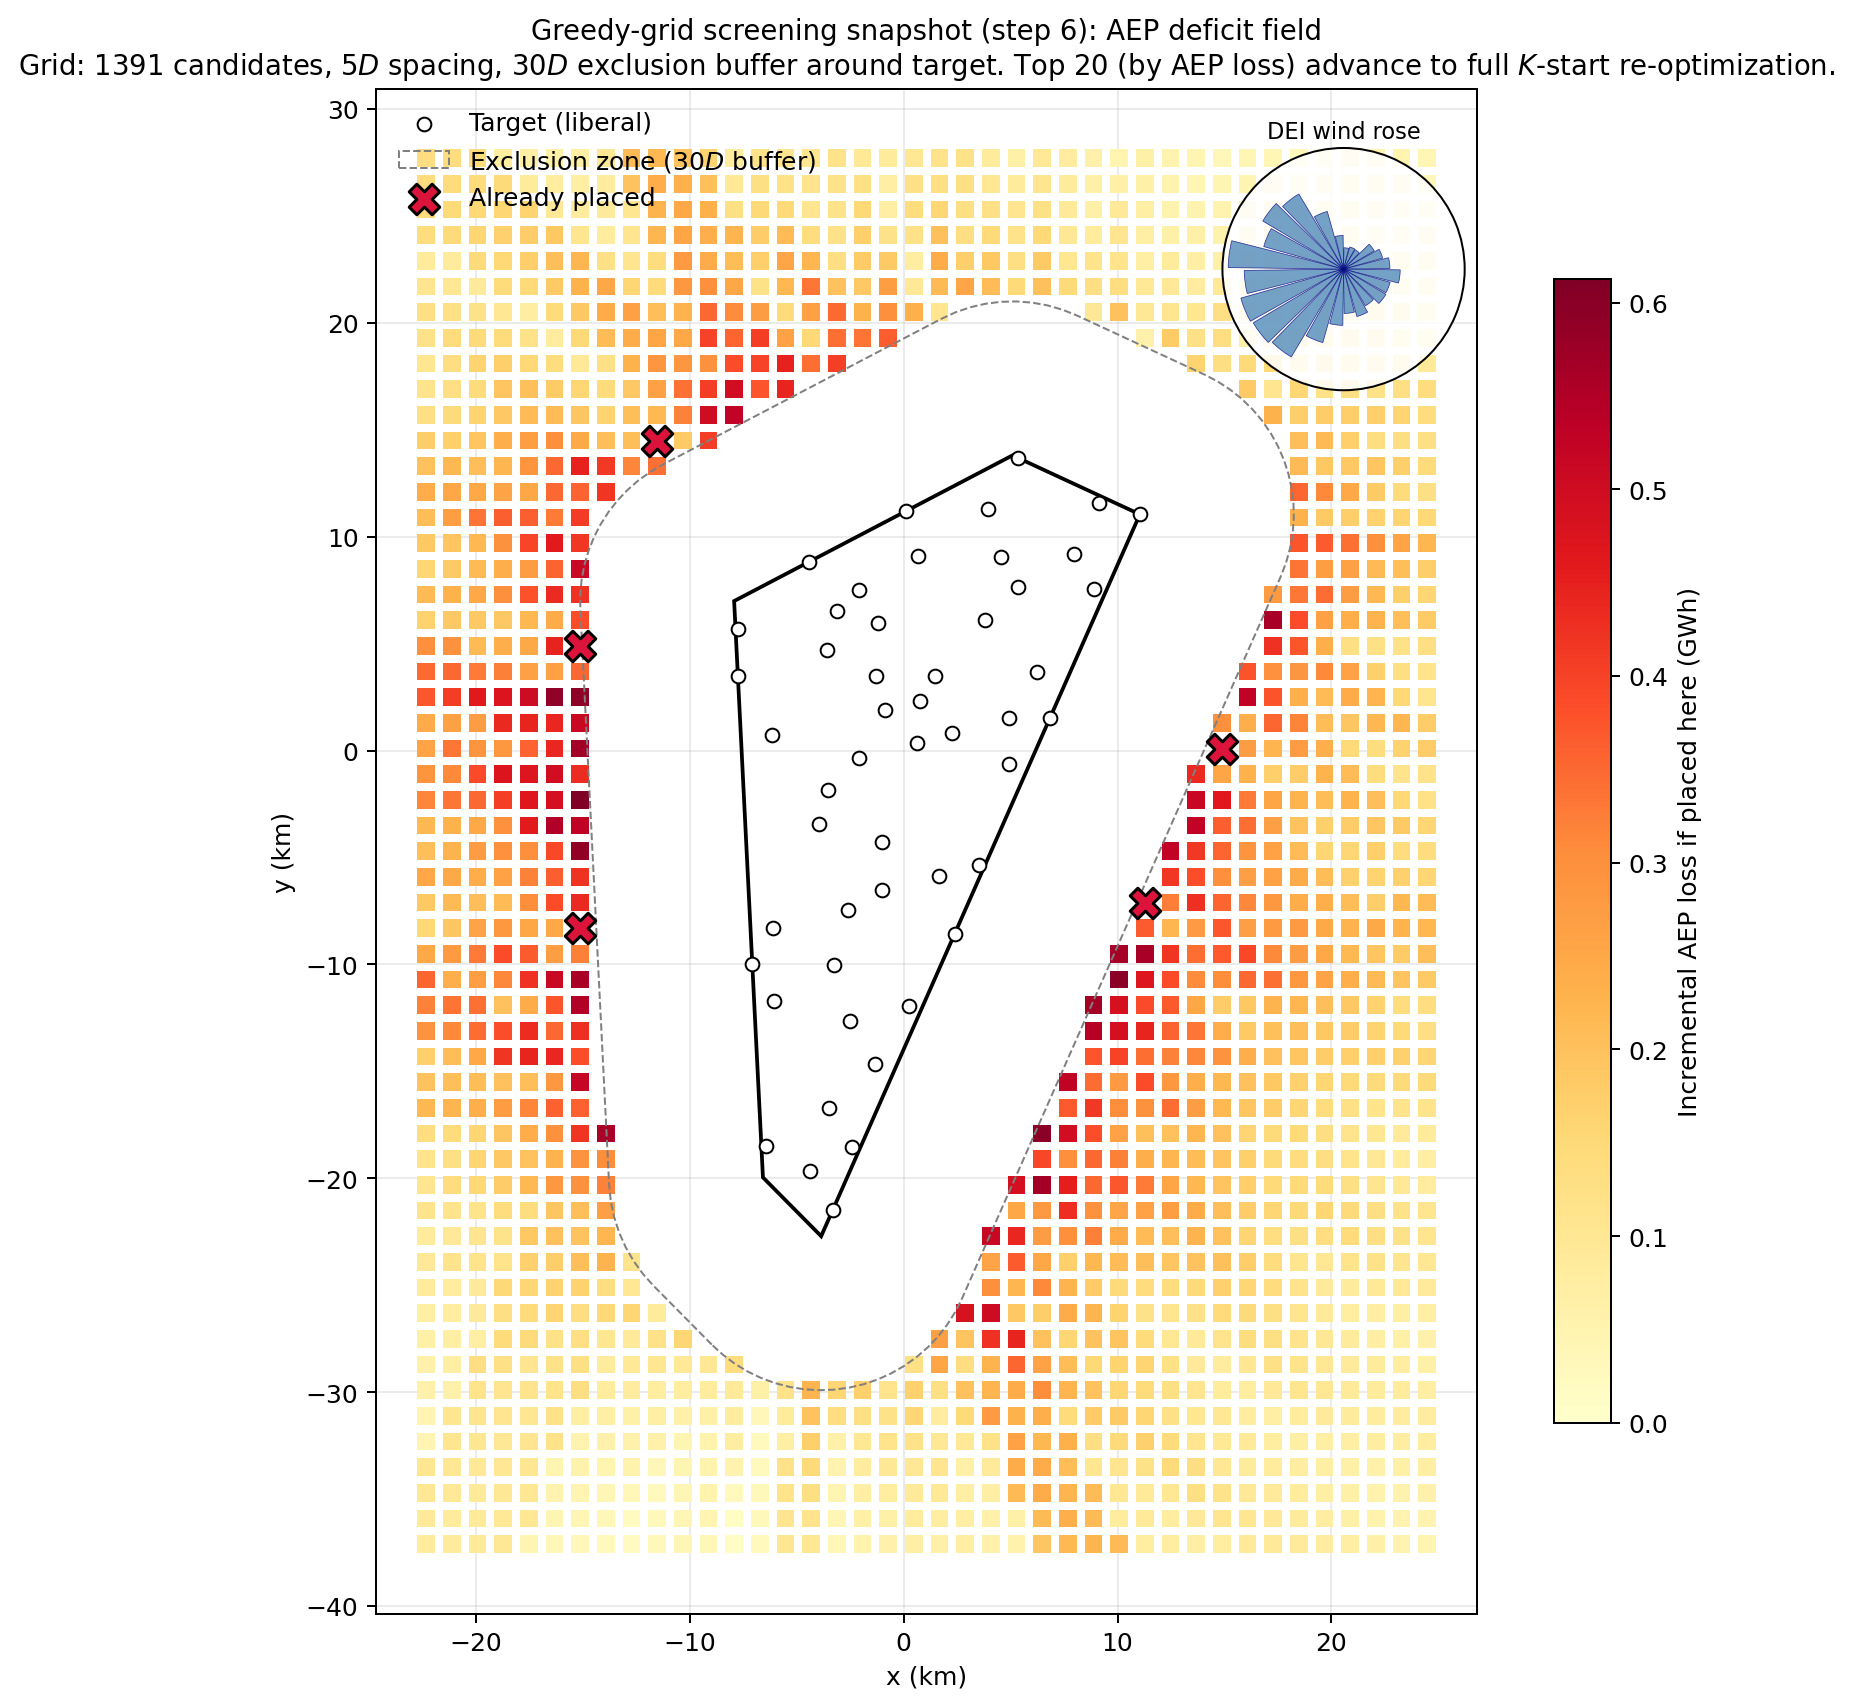
\includegraphics[width=0.85\textwidth]{figures/greedy_screening_snapshot.png}
    \caption{Greedy-grid screening snapshot at step 11/30 (10 neighbors already placed).
    Colored squares: candidate grid (spacing $5D$, extent $30D$ beyond target boundary), colored by the incremental AEP loss that placing a neighbor at that grid point would induce on the liberal target layout (single forward sim, no optimization).
    Red X markers: neighbors already placed in prior steps.
    Only the top 20 candidates by screening AEP loss advance to full $K$-start re-optimization in Stage 2.
    Dashed gray: $2D$ exclusion zone around the target polygon.
    White circles: target liberal layout.}
    \label{fig:greedy-screening}
\end{figure}

This adversarial approach places unconstrained individual turbines---not realistic wind farms---and is designed to find the \emph{maximum achievable regret} for a given wind rose.
It provides an upper bound because: (i)~individual turbines operate at full thrust coefficient, whereas turbines within a real neighboring farm would experience internal wake losses; and (ii)~the greedy algorithm optimizes placement purely to damage the target, whereas a real developer would optimize for their own production.
The results from this analysis should be interpreted as the ceiling on design regret, not as a prediction of what a realistic neighbor would cause.

\subsection{Regret cross-sections: realistic neighbor scenario}\label{sec:cross-section-method}

To assess design regret under more realistic conditions, we introduce the \emph{regret cross-section}.
An identical copy of the target farm---with the same number of turbines, boundary polygon, and liberal-optimized layout ($K_\text{lib} = 300$)---is placed at each combination of 24 bearings ($15$$^\circ$ steps) and 7 buffer distances (2, 5, 10, 15, 20, 30, 40$D$), producing 168 evaluations per wind rose case (Fig.~\ref{fig:radar-schematic}).

\paragraph{Inter-farm distance definition.}
Buffer distance is defined as the minimum Euclidean distance between the boundary polygons of the target and reference farms (not centroid-to-centroid).
For each (bearing, distance) pair, we iteratively compute the centroid offset required to achieve the specified boundary gap, accounting for the irregular polygon shape.
At each configuration, we also record the minimum turbine-to-turbine distance between the two farms.
This boundary-gap definition ensures that no turbines from the reference farm overlap the target farm area at any bearing or distance, which is critical for physically meaningful results.

\paragraph{Reference farm construction.}
The reference farm is an identical translated copy of the target: same boundary polygon, same number of turbines ($N_t = 50$), and same liberal-optimized layout.
This represents the most natural ``what-if'' scenario: a neighboring developer builds the same farm design nearby.

At each position, the target farm is re-optimized with $K = 300$ restarts (matching $K_\text{lib}$) while the reference farm remains fixed.
The resulting polar map separates bearing and distance effects and reveals whether vulnerability is isotropic or directionally concentrated.

\begin{figure}[htbp]
    \centering
    
\includegraphics[width=0.65\textwidth]{figures/radar_schematic.png}
    \caption{Regret cross-section methodology.
    Left: the target farm (gray polygon with blue turbines) surrounded by example reference farm placements at four bearings.
    Buffer distance is measured between polygon boundaries, not centroids.
    Right: the resulting polar regret map, with wind rose inset.}
    \label{fig:radar-schematic}
\end{figure}

\subsection{Multistart optimization and convergence}

Each layout optimization uses gradient-based stochastic gradient descent (SGD) \citep{Quick2023sgd} with a constant learning rate phase followed by a decay phase.
The convergence study (Section~\ref{sec:convergence}) sweeps iteration counts from 100 to 10000 at $K = 500$ starts and finds that regret stabilizes by 2000 total iterations (within 5\% of the 10000-iteration value for all configurations tested).
Production cross-section runs therefore use 2000 iterations; the greedy grid sweep uses 5000 iterations for additional margin.

Restarts include grid initialization, the liberal layout (ensuring regret pooling), and random polygon-sampled positions.
The liberal layout is included as a conservative candidate to guarantee non-negative regret by construction.
Following the convergence analysis of \citet{Quick2026omae}, who found $\sim$400 starts needed for 66-turbine liberal layout convergence, we perform a dedicated convergence study for the regret computation (Section~\ref{sec:convergence}).

Production configurations: $K = 500$ for the greedy grid sweep and buffer analysis (upper bound); $K_\text{lib} = K_\text{cons} = 300$ for cross-sections (realistic scenario), with equal $K$ for liberal and conservative to avoid optimization asymmetry artifacts.


\section{Results}\label{sec:results}

\subsection{Convergence study: how many starts are enough?}\label{sec:convergence}

We sweep $K$ from 1 to 2000 for three configurations spanning the wind rose space (Table~\ref{tab:convergence}, Fig.~\ref{fig:convergence}).
A $5 \times 5$ reference neighbor farm is placed at a fixed bearing and distance for each.

\begin{figure}[htbp]
    \centering
    
\includegraphics[width=\textwidth]{figures/convergence.png}
    \caption{Convergence of design regret with multistart depth~$K$.
    Dashed gray: converged value ($K = 2000$).
    All configurations stabilize by $K \approx 300$.}
    \label{fig:convergence}
\end{figure}

\begin{table}[htbp]
    \centering
    \caption{Design regret (GWh/yr) at selected $K$ values.}
    \label{tab:convergence}
    \begin{tabular}{lcccc}
        \toprule
        Configuration & $K{=}100$ & $K{=}300$ & $K{=}500$ & $K{=}2000$ \\
        \midrule
        Conc.\ unidir.\ ($5D$)  & 15.9 & 26.2 & 26.2 & 26.6 \\
        Conc.\ unidir.\ ($20D$) & 67.9 & 79.3 & 79.3 & 79.3 \\
        Mod.\ bidir.\ ($5D$)    & 43.1 & 43.6 & 43.6 & 43.6 \\
        \bottomrule
    \end{tabular}
\end{table}

At $K = 100$, the concentrated unidirectional case at $5D$ still underestimates regret by $\sim$40\,\%, because the landscape has many local optima with similar standalone AEP but different neighbor-present AEP.
All configurations stabilize by $K = 300$.
SGD iteration convergence is much faster: at $K = 500$, regret at 5000 iterations is within 3\,\% of the 10000-iteration value.

The root cause is catastrophic cancellation: regret is a \emph{difference} between two large AEP values, so a 0.5\,\% error in either optimization can produce a 50\,\% error in regret.
This applies to any study computing AEP differences between strategies---robust optimization, Pareto analysis, or inter-farm coordination assessments.

\subsection{Wind rose shape controls design regret}\label{sec:shape}

Figure~\ref{fig:heatmap} shows design regret across the $(a, f)$ space at $K = 500$.
Regret ranges from 17.2\,GWh (0.4\,\% of AEP) at $a = 0.5$, $f = 0.0$ to 100.6\,GWh (2.5\,\%) at $a = 0.9$, $f = 1.0$---a six-fold range.

\begin{figure}[htbp]
    \centering
    
\includegraphics[width=\textwidth]{figures/edrose_heatmap_k500.png}
    \caption{Design regret across the wind rose shape space at $K = 500$.
    Left: absolute (GWh/yr).
    Right: relative (\% of AEP).
    Markers show fitted parameters for real North Sea sites: DEI (cyan square), Horns Rev~1 (green diamond), Lillgrund (magenta triangle), Borssele (yellow circle), and Princess Amalia (white pentagon).
    All real sites fall in the moderate-regret region of the shape space.}
    \label{fig:heatmap}
\end{figure}

The folding parameter $f$ is the dominant factor (Fig.~\ref{fig:regret_vs_f}).
Mean regret increases monotonically from 45.2\,GWh at $f = 0$ to 77.9\,GWh at $f = 1$.
Concentration ($a$) has a weaker, non-monotonic effect.

\begin{figure}[htbp]
    \centering
    
\includegraphics[width=0.65\textwidth]{figures/regret_vs_f.png}
    \caption{Regret vs.\ folding $f$ at each concentration $a$ ($K = 500$).
    Monotonic increase with $f$ is consistent across all~$a$.}
    \label{fig:regret_vs_f}
\end{figure}

Unidirectional wind ($f = 1$) creates a single wake corridor that the liberal layout is blind to; the conservative optimizer shifts turbines laterally to escape it.
Under bidirectional conditions ($f = 0$), wakes arrive from opposing directions and no lateral shift helps---regret is inherently limited.

For North Sea planning, this means that sites with strongly unidirectional southwesterly winds (characteristic of the German Bight and southern North Sea) face higher design regret than sites with more bidirectional conditions (such as Danish waters).
The DEI wind rose ($a \approx 0.64$, $f \approx 0.38$) falls in the moderate-regret region, consistent with the negligible tradeoffs found by \citet{Quick2026omae}.

\subsection{Buffer distance modulates regret}\label{sec:buffer}

Figure~\ref{fig:buffer} shows regret vs.\ buffer distance at $K = 500$ for three wind roses.

\begin{figure}[htbp]
    \centering
    
\includegraphics[width=0.8\textwidth]{figures/buffer_decay_k500.png}
    \caption{Regret vs.\ buffer distance at $K = 500$, expressed as \% of liberal AEP.
    The NYSERDA 4\,nmi recommendation is marked.}
    \label{fig:buffer}
\end{figure}

For concentrated unidirectional wind ($a = 0.9$, $f = 1.0$), regret drops from 2.5\,\% at $2D$ to 0.4\,\% at $40D$ (9.6\,km).
The bidirectional case ($a = 0.5$, $f = 0.0$) shows gentle decay from 0.4\,\% to 0.2\,\%.

The NYSERDA 4\,nmi ($\sim$$31D$) recommendation reduces regret to $<$1\,\% for all wind roses tested, but is unnecessarily conservative for bidirectional sites.
Wind-rose-dependent buffer standards could allow denser development at low-risk sites (bidirectional, e.g., DEI) while maintaining protection at high-risk sites (unidirectional, e.g., German Bight).
This is directly relevant to the emerging cross-border coordination frameworks for the North Sea \citep{Fliegner2025}.

\subsection{Directional vulnerability: regret cross-sections}\label{sec:cross-sections}

The greedy grid search (Sections~\ref{sec:shape}--\ref{sec:buffer}) establishes an adversarial upper bound by placing individual unconstrained turbines.
To assess regret under more realistic conditions, we now turn to the regret cross-sections, in which an identical copy of the target farm is placed at controlled boundary-gap distances around the target (Section~\ref{sec:cross-section-method}).

\paragraph{Single-direction stress test.}
We begin with the simplest illustrative case: a degenerate wind rose in which all energy arrives from a single sector (90$^\circ$, i.e.\ wind from the east).
Figure~\ref{fig:unidir-aep-loss} presents this case on its own color scale because peak regret (1.25\,\% of AEP) is roughly an order of magnitude above any multi-directional value we encounter below.
The right panel shows design regret; the left panel shows raw AEP loss (liberal layout evaluated with the neighbor, no re-optimization), which separates the neighbor's physical damage from the portion a neighbor-aware layout can avoid.
The radar serves as a methodology check: regret is precisely zero for all downwind bearings (225--315$^\circ$), as it must be when the neighbor casts no wake over the target.
Peak regret occurs at bearings flanking the inflow (75$^\circ$, 105$^\circ$); the dip directly upwind (90$^\circ$) reflects that the liberal layout is already pre-adapted to self-wake from that direction, whereas a slightly off-axis neighbor introduces corridor asymmetry that lateral re-optimization can partially escape.

A second, more surprising feature: the southeast quadrant retains non-trivial regret out to $40D$ (0.37\,\% at 135$^\circ$/$40D$).
At this configuration the neighbor induces 0.44\,\% AEP loss, of which regret captures 0.37\,\%---so re-optimization avoids $\sim$84\,\% of the damage.
Figure~\ref{fig:unidir-flow} shows the flow field: with wind from the east, the SE neighbor's wakes propagate westward and graze the target's southern row even at $40D$.

\begin{figure}[htbp]
    \centering
    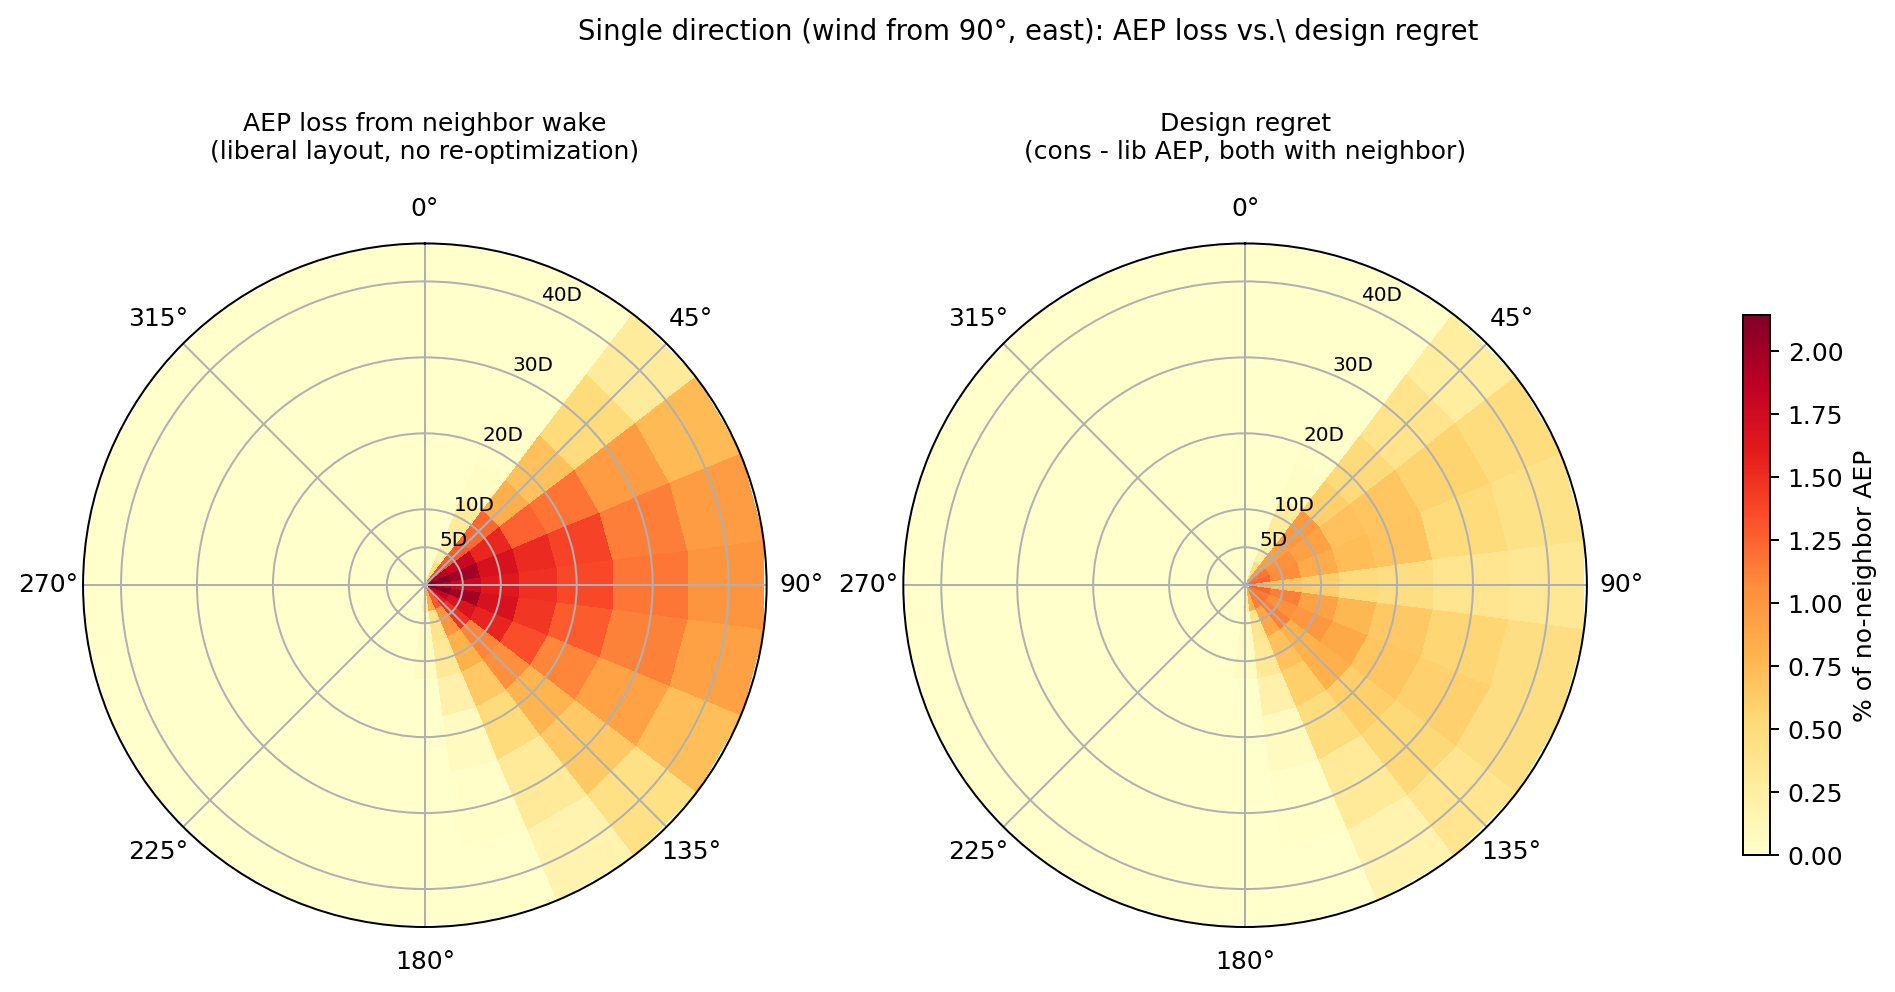
\includegraphics[width=\textwidth]{figures/unidir_aep_loss_vs_regret.png}
    \caption{Single-direction stress test (wind exclusively from 90$^\circ$): AEP loss vs.\ design regret.
    Left: liberal-layout AEP loss due to the neighbor (no target re-optimization).
    Right: design regret (re-optimization benefit).
    Peak regret reaches 1.25\,\% of AEP — roughly ten times larger than any multi-directional case in Fig.~\ref{fig:cross-section}, hence own color scale.
    Downwind bearings (225--315$^\circ$) have zero regret, validating the methodology.}
    \label{fig:unidir-aep-loss}
\end{figure}

\begin{figure}[htbp]
    \centering
    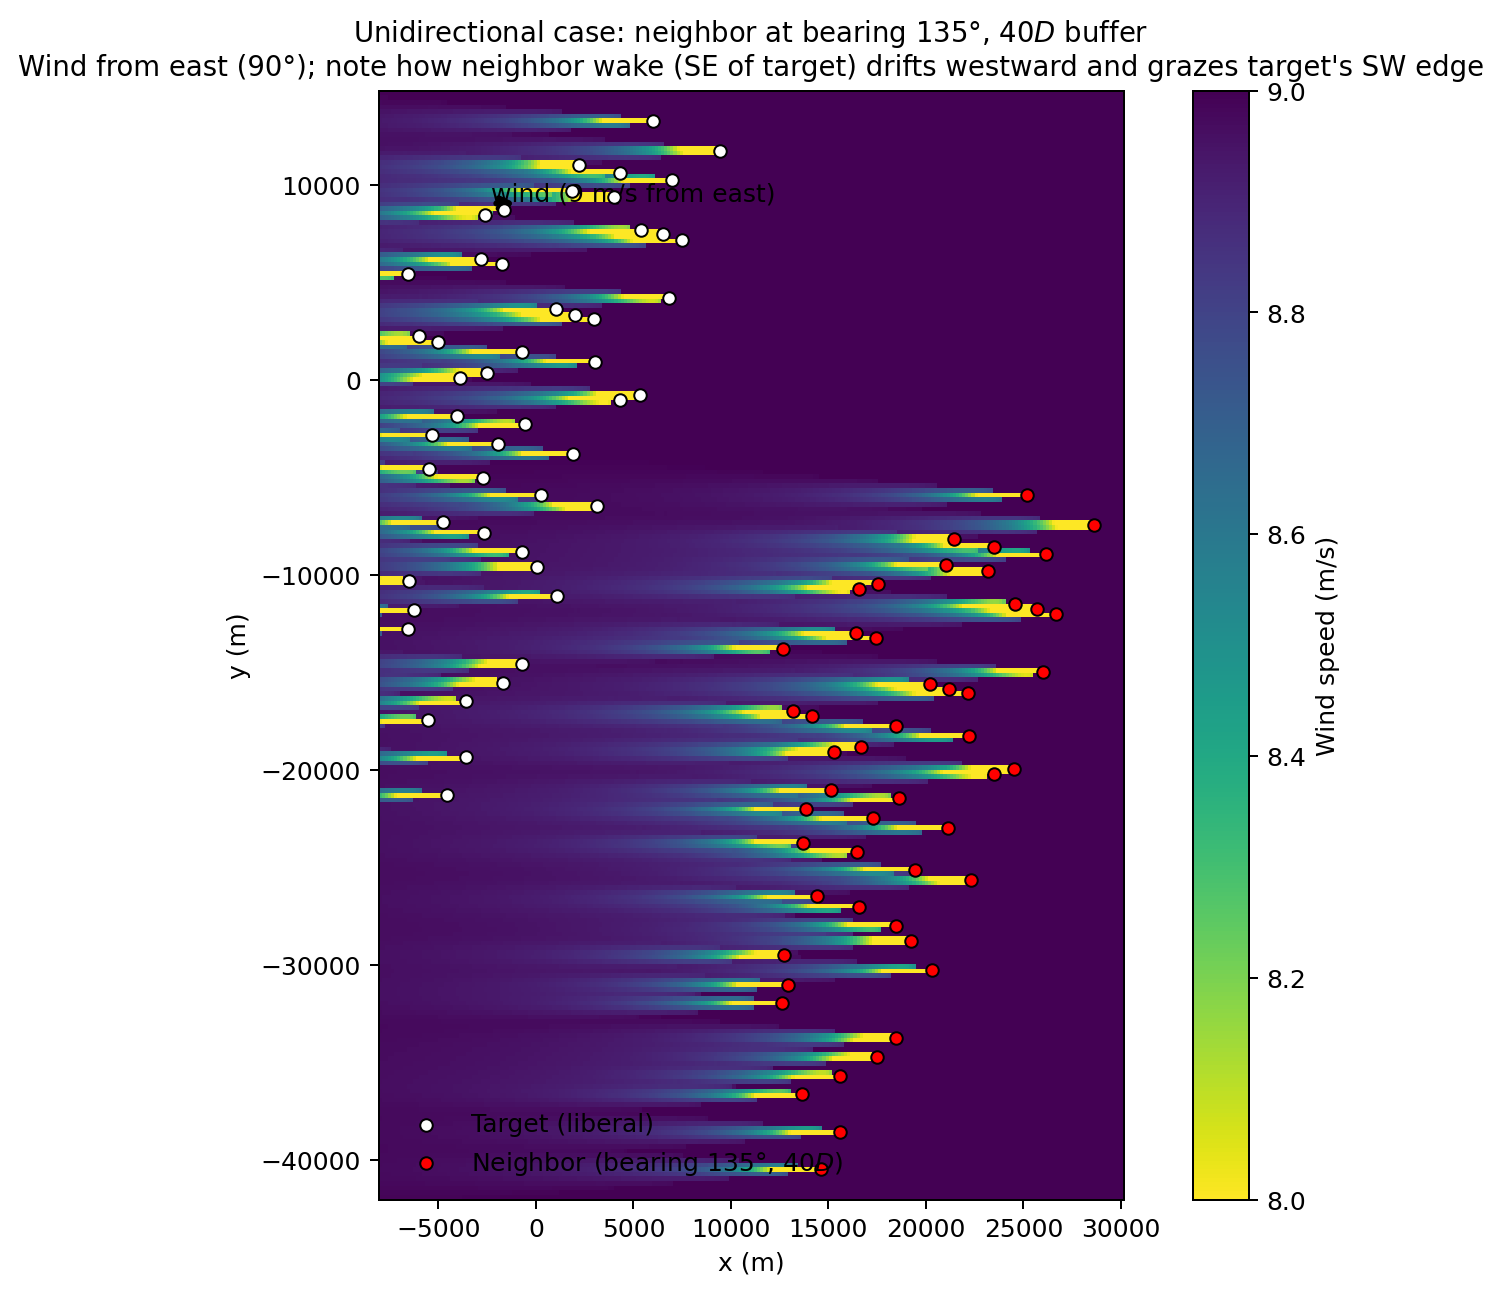
\includegraphics[width=0.75\textwidth]{figures/unidir_flow_135deg_40D.png}
    \caption{Flow field for 135$^\circ$/$40D$ neighbor configuration, single wind direction (9\,m/s from east).
    White circles: target liberal layout.
    Red circles: identical-copy neighbor farm at bearing 135$^\circ$, $40D$ boundary-gap.
    Neighbor wakes propagate westward and intrude on the target's southern turbines, producing the non-trivial SE-quadrant regret observed in Fig.~\ref{fig:unidir-aep-loss}.}
    \label{fig:unidir-flow}
\end{figure}

\paragraph{Realistic multi-directional cases.}
Figure~\ref{fig:cross-section} then presents cross-sections for six multi-directional wind roses at $K_\text{lib} = K_\text{cons} = 300$: the DEI real wind rose and five elliptical parameterizations (Table~\ref{tab:cross-section}).
For all of these, peak regret from a realistic identical neighbor farm is modest: 0.09--0.38\,\% of AEP, with all peaks occurring at the closest buffer distance ($2D$).
This is substantially lower than both the single-direction stress test above and the greedy adversarial upper bound (0.4--2.5\,\% of AEP from Section~\ref{sec:shape}), confirming that both extreme inflow and unconstrained individual turbine placement overstate the risk from a realistic neighboring farm by roughly an order of magnitude.
Regret decays with buffer distance for all cases, reaching negligible levels ($<$0.1\,\%) by 20--40$D$ depending on the wind rose.
The directional pattern is physically intuitive: peak regret aligns with the prevailing upwind direction in most cases, with some angular offset due to the irregular polygon geometry.

\begin{figure}[htbp]
    \centering
    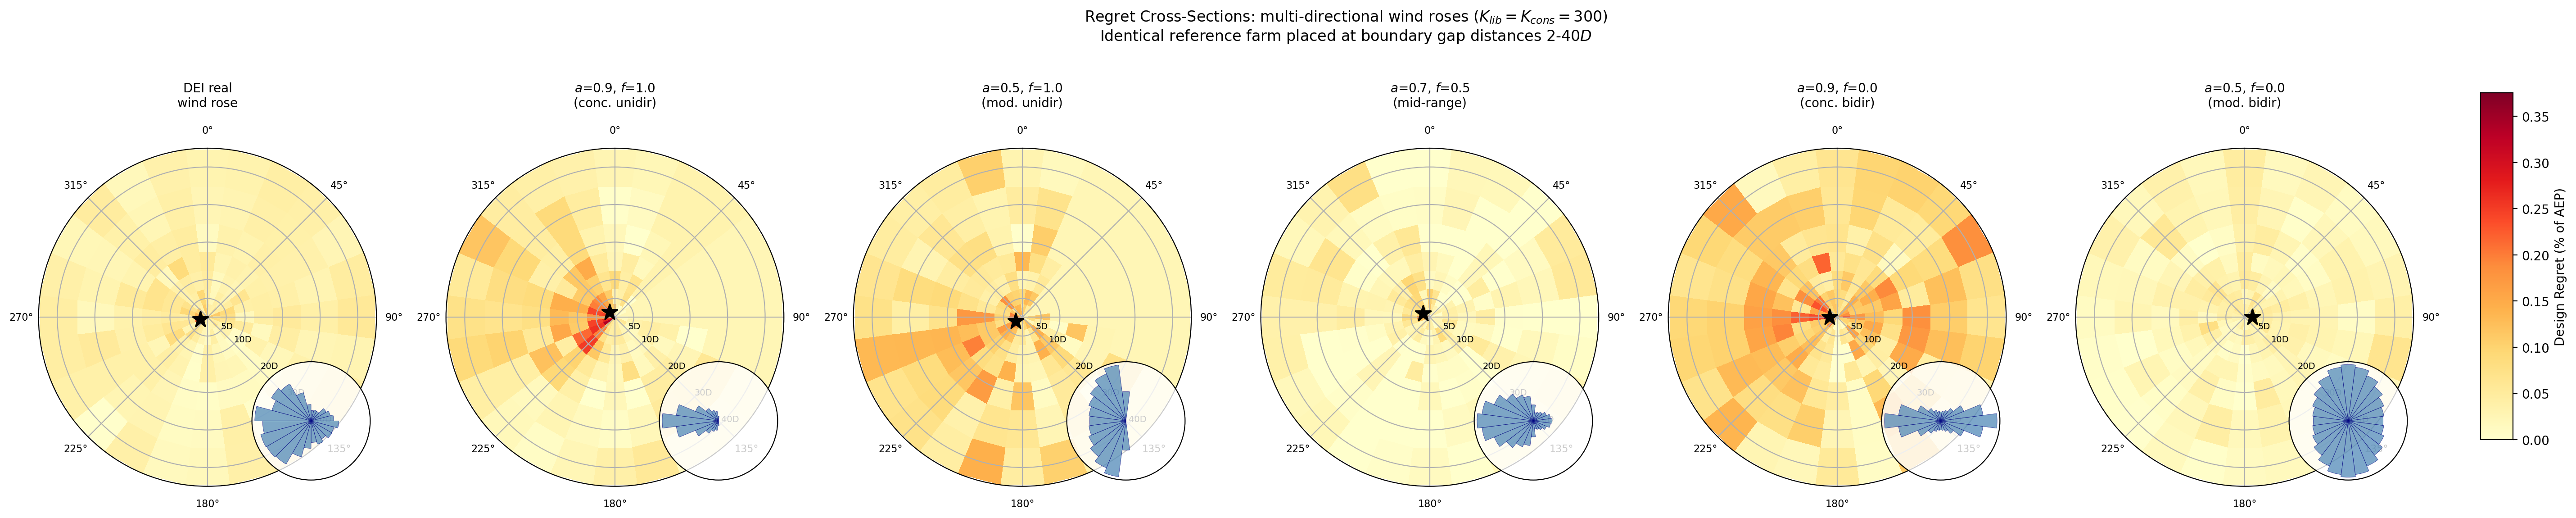
\includegraphics[width=\textwidth]{figures/cross_section_fixed.png}
    \caption{Regret cross-sections for six multi-directional wind roses ($K_\text{lib} = K_\text{cons} = 300$, boundary-gap distances).
    Each panel shows design regret (\% of AEP) as a function of neighbor bearing and buffer distance for an identical copy of the target farm.
    Stars mark peak regret.
    Inset wind roses show the sector frequency distribution.
    All panels share the same color scale.}
    \label{fig:cross-section}
\end{figure}

\begin{table}[htbp]
    \centering
    \caption{Peak regret from cross-sections ($K_\text{lib} = K_\text{cons} = 300$, boundary-gap distance).
    The single-direction case is reported separately because its regret is roughly an order of magnitude larger than any multi-directional case.}
    \label{tab:cross-section}
    \begin{tabular}{lrrrr}
        \toprule
        Case & Max (GWh) & Max (\%) & Bearing & Buffer \\
        \midrule
        \multicolumn{5}{l}{\emph{Single-direction (stress test)}} \\
        Single direction (from E) & 50.5 & 1.25 & 105$^\circ$ & $2D$ \\
        \midrule
        \multicolumn{5}{l}{\emph{Multi-directional (realistic)}} \\
        DEI real wind rose        & 12.4 & 0.22 & 255$^\circ$ & $2D$ \\
        $a = 0.9$, $f = 1.0$     & 13.5 & 0.34 & 315$^\circ$ & $2D$ \\
        $a = 0.5$, $f = 1.0$     &  9.0 & 0.23 & 240$^\circ$ & $2D$ \\
        $a = 0.7$, $f = 0.5$     &  7.8 & 0.20 & 300$^\circ$ & $2D$ \\
        $a = 0.9$, $f = 0.0$     & 14.9 & 0.38 & 270$^\circ$ & $2D$ \\
        $a = 0.5$, $f = 0.0$     &  3.6 & 0.09 &  90$^\circ$ & $2D$ \\
        \bottomrule
    \end{tabular}
\end{table}

\paragraph{$a$-ablation and the geometry of the elliptical rose.}
To trace how regret varies with rose concentration, Figure~\ref{fig:bearing-sweep} sweeps $a$ from 0.01 to 0.9 at fixed full folding ($f = 1$), with the DEI real rose overlaid for reference.
The parameterization has a non-obvious structure: $a = 1/\sqrt{\pi} \approx 0.564$ gives a uniform rose; $a > 0.564$ elongates the ellipse along the prevailing direction, concentrating energy there (at $a = 0.9$, $f = 1$, 20.6\,\% of energy arrives from 270$^\circ$); $a < 0.564$ elongates it perpendicular to the prevailing direction, producing a bimodal rose with peaks at $\theta_\text{prev} \pm 90^\circ$ (at $a = 0.01$, $f = 1$, $\sim$50\,\% each at 0$^\circ$ and 180$^\circ$).
Small $a$ therefore does not approximate the single-sector stress test; it represents a distinct perpendicular-bimodal regime.
Regret reflects this: tiny $a$ (0.01--0.05) reaches 1.5--1.8\,\% at $2D$ because the target faces two concentrated inflow axes; moderate $a$ (0.3--0.5, near-uniform) sits at 0.1--0.3\,\%; and $a = 0.9$ (concentrated westerly) yields $\sim$0.3\,\%.
Realistic North Sea wind climates sit in the moderate-$a$ valley.
The perpendicular-bimodal and single-sector corners of the rose space both produce $\geq$1\,\% regret, but they represent physically distinct wind climates; neither is characteristic of operational offshore sites.

\begin{figure}[htbp]
    \centering
    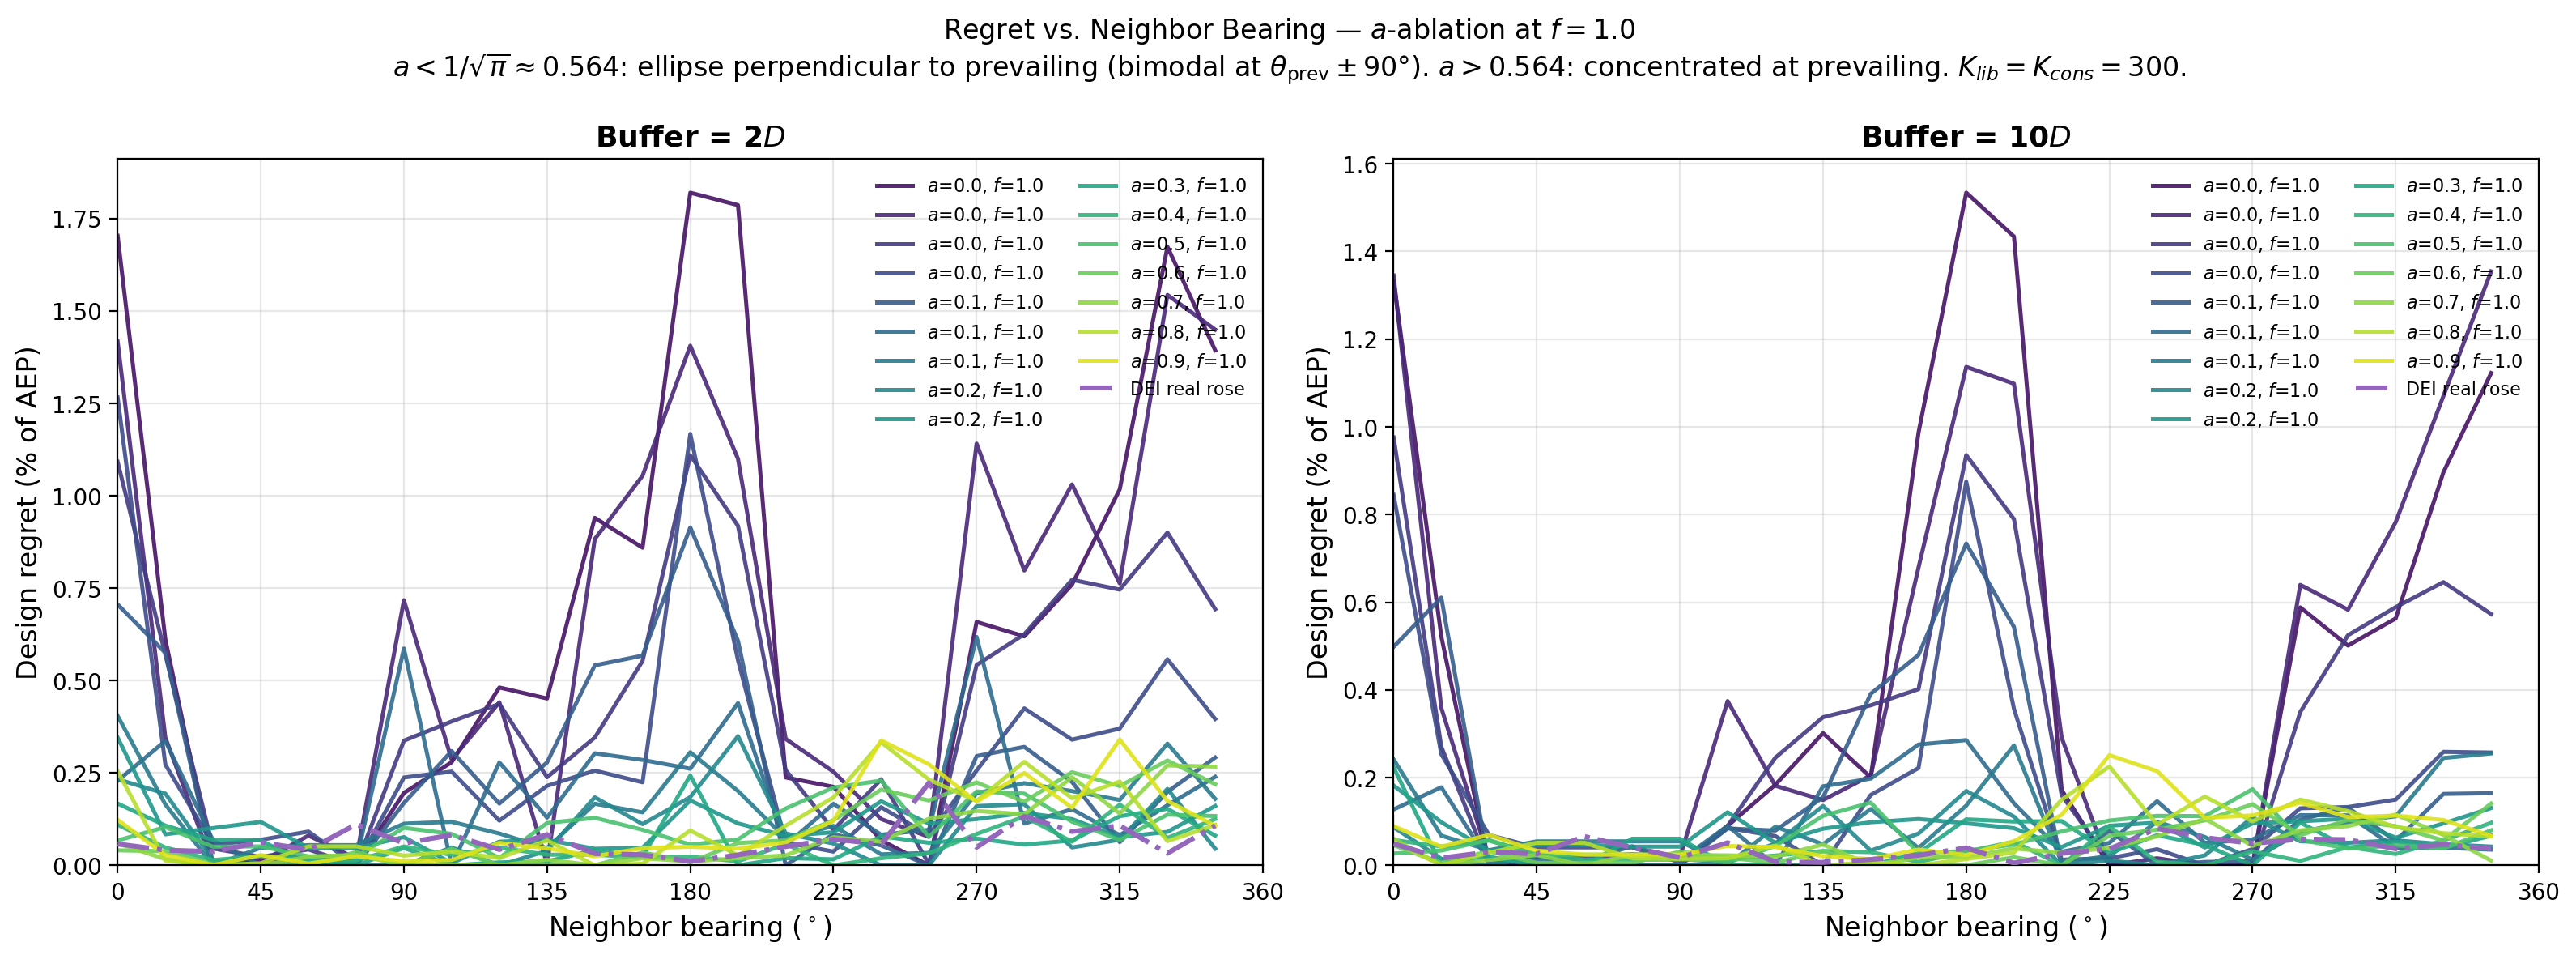
\includegraphics[width=\textwidth]{figures/bearing_sweep.png}
    \caption{Regret vs.\ neighbor bearing as the wind rose transitions from bidirectional to unidirectional.
    Viridis curves: $f$-sweep at fixed $a = 0.9$ (prevailing direction 270$^\circ$).
    Red dashed: pure single-direction at 270$^\circ$.
    Purple dash-dot: DEI real wind rose.
    Black: single-direction at 90$^\circ$ (east-inflow stress test).
    Left: $2D$ buffer; right: $10D$.}
    \label{fig:bearing-sweep}
\end{figure}



\section{Discussion}\label{sec:discussion}

\subsection{Real North Sea sites in the shape space}

To ground the parametric results in real planning decisions, we fit the elliptical model to five North Sea offshore wind sites (Table~\ref{tab:sites}, Fig.~\ref{fig:heatmap}).
All five sites fall in the moderate-regret region of the $(a, f)$ space, with $a \in [0.62, 0.73]$ and $f \in [0.18, 0.54]$.
No operational North Sea site in our sample reaches the high-regret corner ($a > 0.8$, $f > 0.75$), though this does not preclude future lease areas---particularly in the southern North Sea---from doing so.

\begin{table}[htbp]
    \centering
    \caption{Fitted elliptical wind rose parameters for North Sea offshore sites.
    Data sources: Horns Rev~1 and Lillgrund from PyWake; Borssele from IEA Wind Task~55 ROWP; Princess Amalia from the python-windrose package; DEI from 10-year NEWA timeseries.}
    \label{tab:sites}
    \begin{tabular}{lcccl}
        \toprule
        Site & $a$ & $f$ & $\theta_\text{prev}$ & $R^2$ \\
        \midrule
        Horns Rev 1 (DK)       & 0.649 & 0.384 & 240\,$^\circ$ & 0.82 \\
        Lillgrund (SE)          & 0.621 & 0.544 & 236\,$^\circ$ & 0.77 \\
        Borssele (NL)           & 0.728 & 0.291 & 240\,$^\circ$ & 0.87 \\
        Princess Amalia (NL)    & 0.650 & 0.182 & 210\,$^\circ$ & 0.49 \\
        Danish Energy Island    & 0.637 & 0.384 & 251\,$^\circ$ & 0.84 \\
        \bottomrule
    \end{tabular}
\end{table}

The sites cluster in the $(a, f)$ space because North Sea wind climates share a common driver: Atlantic weather systems producing dominant southwesterly winds.
The spread in $f$ (0.18--0.54) reflects varying degrees of bidirectionality, with Princess Amalia showing the most bidirectional character ($f = 0.18$, lowest regret risk) and Lillgrund the most unidirectional ($f = 0.54$, highest regret risk among the five).

\subsection{Implications for North Sea cluster development}

The six-fold variation in design regret across wind rose shape has direct implications for the North Sea's emerging cluster framework.

\paragraph{Economic magnitude.}
For a representative 750\,MW farm (50$\times$15\,MW), design regret of 2.5\,\% corresponds to $\sim$100\,GWh/yr.
At a contract-for-difference strike price of 70\,EUR/MWh, this amounts to $\sim$7\,M EUR/yr, or $\sim$175\,M EUR over a 25-year operational lifetime.
Even at the moderate regret levels observed for real North Sea sites ($\sim$1\,\%), the lifetime cost exceeds 70\,M EUR---comparable to the cost of a single turbine foundation.
By contrast, the marginal cost of running a neighbor-aware layout optimization is negligible relative to project CAPEX.

\paragraph{German Bight and southern North Sea.}
Sites with strongly unidirectional southwesterly winds sit in the high-regret region ($f \gtrsim 0.75$).
Here, the value of coordinated design is highest, and buffer distances of $30$--$40D$ (7--10\,km) may be needed to reduce regret below 1\,\%.
The projected 30\,\% capacity factor reduction from cluster wakes \citep{Fliegner2025} is partially a design problem, not just a physics problem: some of this loss could be mitigated by neighbor-aware layout optimization.

\paragraph{Danish waters.}
The DEI wind rose ($f \approx 0.38$) benefits from a natural resilience: wakes from any single direction are partially offset by energy captured from the opposing direction, limiting the rearrangement advantage of a neighbor-aware design.
This explains the negligible design tradeoffs found by \citet{Quick2026omae}.
However, this resilience is a property of the wind climate, not the farm---other Danish sites with different wind characteristics may not share it.

\paragraph{Cross-border coordination.}
The value of inter-farm coordination is itself wind-rose-dependent.
Our results suggest that coordination frameworks like the ``good neighbour'' principle in the UK EN-3 guidance should be weighted by wind rose directionality.
Fixed buffer distances---such as the NYSERDA 4\,nmi recommendation---are adequate for all sites tested but inefficient: bidirectional sites need only $\sim$$10D$ to achieve the same residual regret.
Wind-rose-conditional buffers could allow denser development at low-risk sites without compromising high-risk ones.

\subsection{The convergence problem}

Our most broadly applicable finding is methodological.
Small multistart budgets---even $K = 100$---can miss substantial regret, and only at $K \geq 300$ does the estimate stabilize.
The cause is catastrophic cancellation: regret is a difference between two large, noisy AEP values.
A 0.5\,\% miss in either optimization can produce a 50\,\% error in the difference.

This affects any study computing AEP differences between strategies.
We recommend $K \geq 300$ for 50-turbine farms and proportionally more for larger farms.
The computational cost at $K = 500$ was approximately 2\,hours per wind rose on a single AMD MI250X GCD, or 70\,GPU-hours for the full 35-case sweep.

\subsection{Limitations}

\paragraph{Wake model.}
We use \citet{Bastankhah2014} with $k = 0.04$ and root-sum-of-squares superposition.
More sophisticated models (e.g., TurbOPark) may change absolute magnitudes.
The qualitative findings---folding dominance, directional vulnerability patterns---depend on wake corridor geometry, not magnitude, and are expected to be robust.

\paragraph{Adversarial vs.\ realistic neighbors.}
The greedy grid search places unconstrained individual turbines, while the cross-section uses a fixed reference farm copy.
Neither represents a self-interested neighbor that optimizes its own AEP.
A self-interested neighbor might concentrate turbines in high-wind upwind positions, potentially producing different regret patterns.
This comparison is left to future work with the corrected boundary-gap methodology.

\paragraph{Constant wind speed.}
Real North Sea sites have speed--direction correlations.
If high-speed winds are concentrated in the dominant direction (common for storm-driven sites), regret could be amplified through the cubic power relationship.

\paragraph{Single farm geometry.}
Results may depend on the DEI polygon shape.
Different boundaries could affect the layout optimization landscape and the potential for lateral escape from wake corridors.

\paragraph{Cross-section resolution.}
The cross-section analysis uses 24 bearings and 7 distances, which may miss fine angular structure in the regret field.


\section{Conclusions}

\begin{enumerate}
    \item \textbf{Reliable regret estimation requires many restarts.}
    Regret stabilizes only by $K = 300$ and does not change through $K = 2000$.
    Any study computing AEP differences between strategies should use $K \geq 300$.

    \item \textbf{Design regret varies six-fold across the wind rose shape space.}
    At $K = 500$, regret ranges from 17\,GWh/yr (0.4\,\%) under bidirectional conditions to 101\,GWh/yr (2.5\,\%) under concentrated unidirectional conditions.
    Folding ($f$, bidirectional vs.\ unidirectional) is the primary driver.

    \item \textbf{Buffer distance requirements are wind-rose-dependent.}
    Concentrated unidirectional sites retain 0.4\,\% residual regret at $40D$ (9.6\,km).
    Bidirectional sites achieve comparable levels at $10D$ (2.4\,km).
    Wind-rose-conditional buffer standards could allow denser North Sea development at low-risk sites.

    \item \textbf{Realistic neighbor regret is an order of magnitude below the adversarial upper bound.}
    An identical neighboring farm placed at boundary-gap distances produces 0.1--0.4\,\% regret for multi-directional wind roses (vs.\ 0.4--2.5\,\% from adversarial individual turbines).
    A degenerate single-direction stress test yields 1.25\,\%, peaking at bearings flanking the inflow direction.
    The directional pattern is physically intuitive and decays with buffer distance.
\end{enumerate}

The Danish Energy Island, with its partially bidirectional wind rose ($f \approx 0.38$), sits in the low-to-moderate regret region.
Sites in the southern North Sea with strongly unidirectional southwesterly winds are substantially more vulnerable.
As North Sea clustering intensifies toward the 300\,GW target, incorporating wind rose directionality into buffer distance standards and coordination frameworks will become increasingly important for efficient maritime spatial planning.


\codedataavailability{
The simulation framework (pixwake) and analysis scripts are available at \url{https://github.com/kilojoules/cluster-tradeoffs}.
The elliptical wind rose parameterization uses the edrose package \citep{Hart2025}, available at \url{https://github.com/kilojoules/edrose}.
}

\authorcontribution{
JQ designed the study, developed the simulation framework, performed all computations, and wrote the manuscript.
SK contributed to methodology and manuscript revision.
PER supervised the research and contributed to methodology and manuscript revision.
}

\competinginterests{
The authors declare no competing interests.
}

\begin{acknowledgements}
Computational resources were provided by the LUMI supercomputer, hosted by CSC -- IT Center for Science (Finland) and the LUMI consortium.
\end{acknowledgements}

\bibliographystyle{copernicus}
\bibliography{references}

\end{document}
